\documentclass[landscape]{article}
\usepackage[a4paper,margin=1.3cm]{geometry}
\usepackage[utf8]{inputenc}
\usepackage[T1]{fontenc}
\usepackage{multicol}
\usepackage{lipsum}
\usepackage{amsmath}
\usepackage{xcolor}

\usepackage{graphicx}
\graphicspath{ {./images/} }

\setlength{\columnsep}{1cm}
\renewcommand{\columnseprulecolor}{\normalcolor}
% set \paragraph vertical spacing
\makeatletter
\renewcommand{\paragraph}{\@startsection{paragraph}{4}{\z@}%
                                    {1.5ex}%
                                    {-0.75em}%
                                    {\normalfont\normalsize\bfseries}}
\makeatother
% reduce space before \subparagraph
\makeatletter
\renewcommand{\subparagraph}{\@startsection{subparagraph}{5}{\z@}%
                                       {1ex}%
                                       {-0.75em}%
                                       {\normalfont\normalsize\bfseries\hspace{1.25em}}}% Add \hspace{1.25em} for 1 level of indent
\makeatother
% add vertical space before \minipage and rename environment to \minipage
\let\oldminipage\minipage
\let\endoldminipage\endminipage
\renewenvironment{minipage}{\vspace{0.5em}\begin{oldminipage}{0.925\linewidth}}{\end{oldminipage}}

% Custom command for paragraph content numbering
% Define counters
\newcounter{num}

% Define the \num command to step the num counter and print the number
\newcommand{\num}{%
    \stepcounter{num}%
    (\thenum) %
}

% Reset the num counter when num is stepped
\newcommand{\snum}{%
    \setcounter{num}{0}%
    \num%
}

% Custom command for horizontal separator
\newcommand{\sep}{\noindent\rule{\linewidth}{0.5pt}}

\pagenumbering{gobble}

\begin{document}

\begin{multicols*}{3}
    \footnotesize % Change the font size here if needed

    \section*{ISI - Sécurité Informatique \\ \small{Leonard Cseres - Mars 2024}}

    \paragraph{Loi Suisse}

    \subparagraph{A.143} \textit{Soustraction de données} : Appropriation intentionnelle et frauduleuse de données protégées.
    \subparagraph{A.143bis} \textit{Accès indu à un système informatique} : Accès non autorisé à des systèmes protégés, avec circulation de données punissable.

    \paragraph{CIA} Préservation de la confidentialité, intégrité et disponibilité de l'information

    \begin{itemize}
        \item \textbf{Confidentialité} : Seule les personnes autorisées peuvent accéder à l'information
        \item \textbf{Intégrité} : Protéger l'exactitude et la complétude de l'information
        \item \textbf{Disponibilité} : L'information est accessible par les personnes autorisées
    \end{itemize}

    \paragraph{SSI} \textit{Prévention}, \textit{Détection}, \textit{Réaction} (analyse et confinement), \textit{Récupération}
    \subparagraph{3 domaines} Sécurité physique, organisationnelle, technique

    \paragraph{5 Couches} \snum\textit{Physique}, \num\textit{Réseau}, \num\textit{Protocoles}, \num\textit{Hosts} (systèmes d'exploitation), \num\textit{Application}

    \paragraph{Contrôle d’accès - AAA} Authentification (identité), Autorisation (droits), Accounting/audit (traçabilité)

    \paragraph{Dommages} Perte de CIA

    \paragraph{5 Principles fondamentaux} \snum\textcolor{blue!80}{Sécurité globale} autant que le maillon le plus faible, \num\textcolor{blue!80}{Sécurité parfaite} impossible, \num\textcolor{blue!80}{Sécurité processus} pas un produit, \num\textcolor{blue!80}{Sécurité complexité} inversement proportionnelle, \num\textcolor{blue!80}{Participation} des utilisateurs

    \paragraph{9 Règles fondamentales} \snum Interdiction par défaut, \num moindre privilège, \num défense en profondeur, \num séparation des fonctions, \num segmentation (diversification), \num économie de mécanismes (simplicité), \num goulet d’étranglement (centralisation), \num interruption/erreur sûre, \num éviter la sécurité (transparence)

    \paragraph{Types de menaces} \textit{Accidentelles}, \textit{Environnementales}, \textit{Délibérées}

    \paragraph{Types de vulnérabilités} \textit{Matérielles}, \textit{Logicielles}, \textit{Réseaux}, \textit{Personnelles}, \textit{Physiques}, \textit{Organisation}

    \sep

    \paragraph{Craquage de mot de passe} \textit{Brute force}, \textit{Dictionnaire}, \textit{Heuristique} (variations d'un dictionnaire), \textit{Pré-génération}

    \begin{equation*}
        N = \text{Alphabet}^{\text{Taille}} \qquad T_{moy} = \frac{N}{2}
    \end{equation*}

    \paragraph{Rainbow table} Table de hachage pré-calculée (évite les collisions et optimise la probabilité de succès et le stockage)

    \paragraph{Windows} \texttt{c:\textbackslash Windows\textbackslash system32\textbackslash config\textbackslash SAM}

    \paragraph{Linux} \texttt{/etc/passwd} et \texttt{/etc/shadow} (root), sous forme \texttt{\$type\$salt\$hash}

    \paragraph{LM/NTLM} Protocole d'auth. de Microsoft (pas salé) \snum\textbf{LAN \& LM}: Win 9x/ME, \num\textbf{LM \& NTML}: Win NT/2K/XP/2003, \num\textbf{NTLM}: Win Vista/7/8/10/11

    \sep

    \paragraph{Protection messagerie} Utiliser des protocoles sécurisés (TLS), utiliser la messagerie sécurisée (PGP, GPG)

    \paragraph{Maliciel} Logiciel malveillant
    \begin{itemize}
        \item \textbf{Virus} S'attache à d'autres programmes ou fichiers, on besoin de l'intervention de l'utilisateur pour se propager
        \item \textbf{Ver} Se propage via les réseaux et tout seul
        \item \textbf{Spyware} Collecte des informations sur l'utilisateur
        \item \textbf{Trojan} Se fait passer pour un logiciel légitime
        \item \textbf{Ransomware} Crypte et demande une rançon
    \end{itemize}

    \paragraph{Protection maliciels} Vérification sur VirusTotal, antivirus, patch, backups, éducation

    \begin{multicols*}{2}
        \paragraph{Pillage} Vol d'informations et/ou d'argent

        \paragraph{Backdoor} Programme qui permet à des personnes non autorisées d'accéder à un système (introduit par un exploit, virus, ver, trojan, etc.)

        \paragraph{RootKit} Maliciel qui modifie le système d'exploitation pour cacher sa présence

        \begin{minipage}
            \centering
            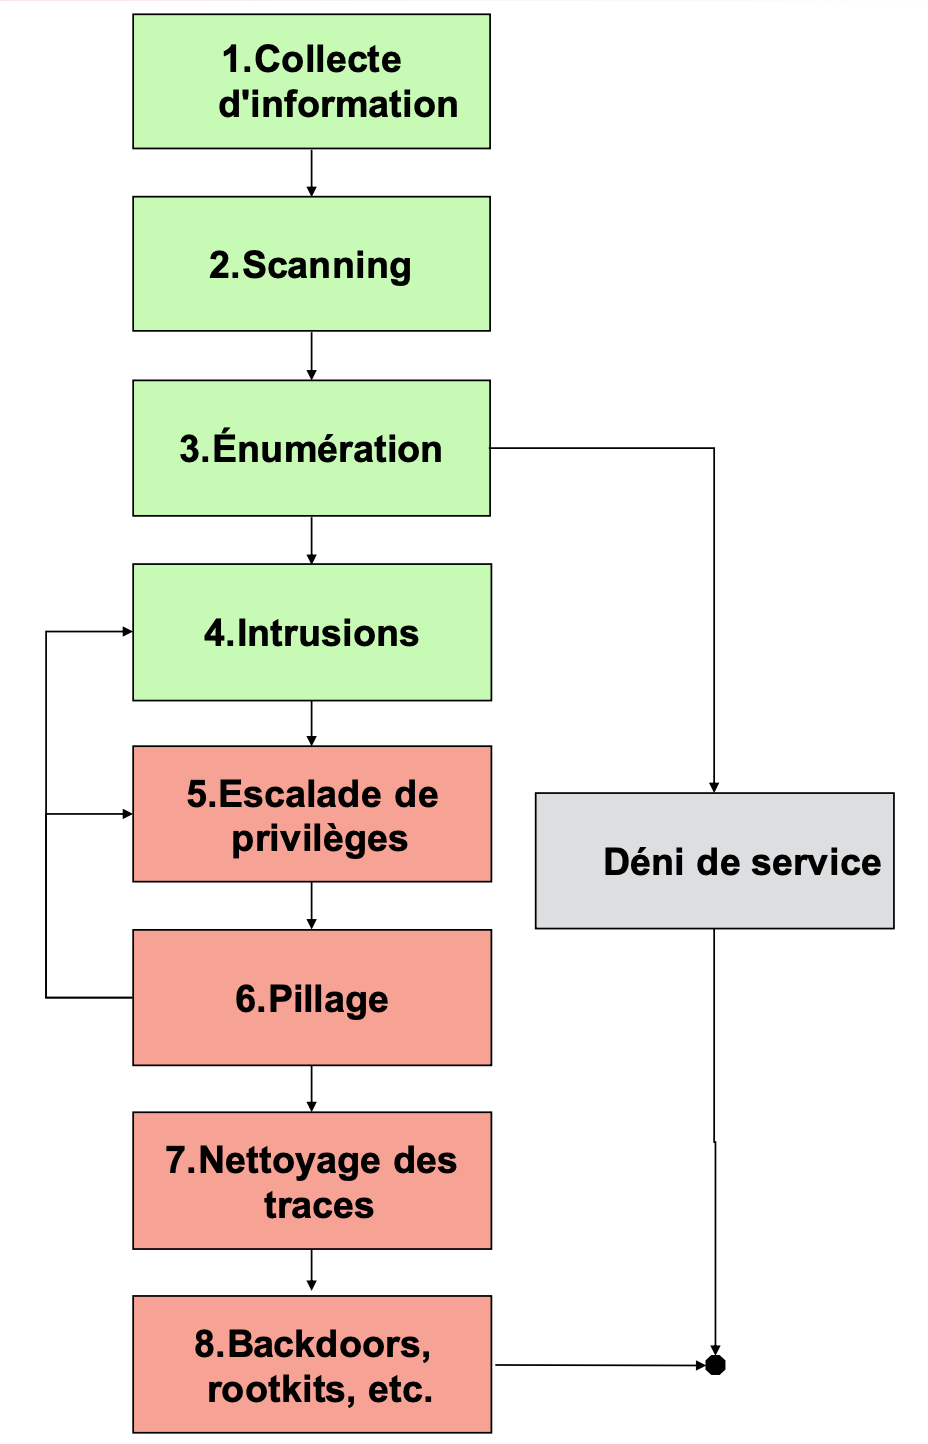
\includegraphics[width=\linewidth]{attaque.png}
        \end{minipage}
    \end{multicols*}

    \paragraph{Protocoles HTTP}
    \begin{verbatim}
    GET /index.html HTTP/1.1
    Host: www.example.com
    HTTP/1.1 200 OK
    Content-Type: text/html
    \end{verbatim}\vspace{-1em}

    \subparagraph{Communication} \textit{Basique} (port TCP/UDP), \textit{Évoluée} (canal caché + chiffré comme ICMP ping ou DNS), \textit{Avancée} (injecte DLL et passe par IE pour aller chercher périodiquement ses ordres)

    \begin{minipage}
        \centering
        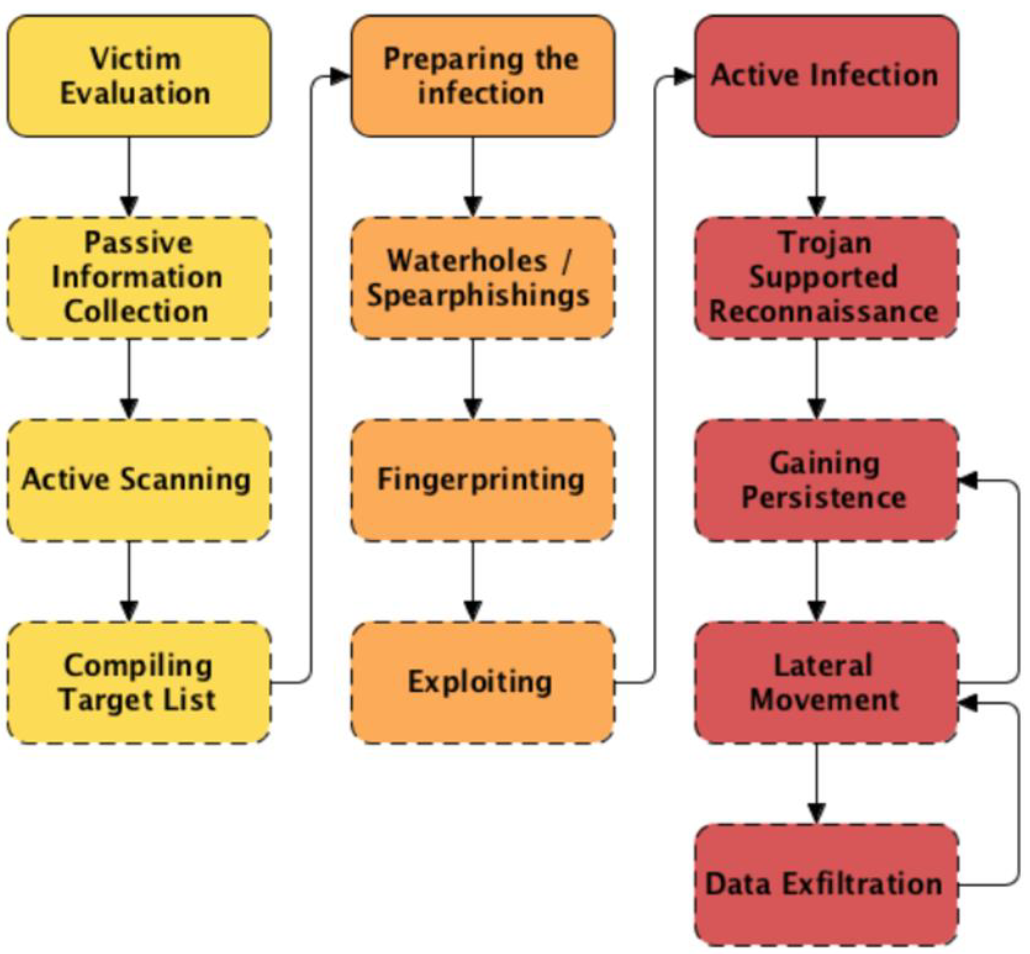
\includegraphics[width=0.6\linewidth]{ruag.png}
    \end{minipage}

    % TODO: Add lockbit and other companies
    % TODO: Hash pour verifier si une fichier a été modifié

    \sep

    \paragraph{Attaques Web} \snum\textcolor{blue!80}{Parcours d'arborescence}, \num\textcolor{blue!80}{Contournement côté client} (cookies), \num\textcolor{blue!80}{XSS} (Cross-Site Scripting) \textit{Reflected}: injecté dans l'URL, \textit{Stored}: injecté dans la base de données, \textit{DOM-based}: injecté dans le DOM, \num\textcolor{blue!80}{Injection SQL}, \num\textcolor{blue!80}{CSRF} (Cross-Site Request Forgery) forcer actions indésirées, \num\textcolor{blue!80}{Clickjacking}

    \paragraph{Prévention}
    \begin{itemize}
        \item Utilisation de requêtes préparées (prepared statements)
        \item Échappement des caractères spéciaux dans les entrées utilisateur (sanitation)
        \item Limitation des permissions des comptes de base de données utilisés par l'application
        \item Utilisation d'en-têtes de sécurité (e.g., Content Security Policy)
        \item \textbf{SAST} Static Application Security Testing (ex: \textit{Semgrep})
        \item \textbf{DAST} Dynamic Application Security Testing (ex: \textit{ZAProxy})
    \end{itemize}

    \paragraph{Sécurité OWASP}
    \begin{itemize}
        \item \textbf{Top 10} \snum Broken Access Control \num Cryptographic Failures \num Injection \num Insecure Design \num Security Misconfiguration \num Vulnerable and Outdated Components \num Identification and Authentication Failures \num Software and Data Integrity Failures \num Security Logging and Monitoring Failures \num Server-Side Request Forgery
        \item \textbf{Juice Shop} Un environnement vulnérable pour s'entraîner
    \end{itemize}

    \sep

    \paragraph{Cryptographie} Apporte la \textit{Confidentialité}, \textit{Authenticité}, \textit{Intégrité} (pas de modification), \textit{Non-répudiation} (ne peut pas nier de qui vient l'information)
    \begin{itemize}
        \item Cryptanalyse (décrypter une information sans connaître a priori la clé)
        \item Cryptologie (étude de la cryptographie et de la cryptanalyse)
    \end{itemize}

    \paragraph{Principe de Kerchhoff} La sécurité d'un système cryptographique doit reposer sur la confidentialité de la clé et non sur celle de l'algorithme (sécurité par l'obscurité)

    \paragraph{Algorithme de chiffrement/déchiffrement}
    \begin{itemize}
        \item Cipher (clé symétrique/secrète)
        \item PK (clé asymétrique/publique)
    \end{itemize}

    \paragraph{Confidentialité parfaite} L'adversaire ne peut rien apprendre de l'information chiffrée (jamais vrai en pratique)

    \paragraph{Block Cypher} Permutation mathématique d'un bloc de données en un autre bloc de même taille (opération inversible)
    \paragraph{Stream Cypher} Chiffrement bit à bit (opération non-inversible)

    \paragraph{DES} Block cypher de 64 bits avec une clé de 56 bits
    \subparagraph{Faiblesse} $2^{56}$ clés possibles, trop facile à casser
    \subparagraph{3key-TDES} $DES \rightarrow DES^{-1} \rightarrow DES$ ($-1$ garde la rétro-compatibilité)

    \paragraph{AES} Block cypher de 128 bits avec une clé de 128, 192 ou 256 bits

    \paragraph{Modes de chiffrement}\mbox{}\\\\
    \begin{minipage}
        \centering
        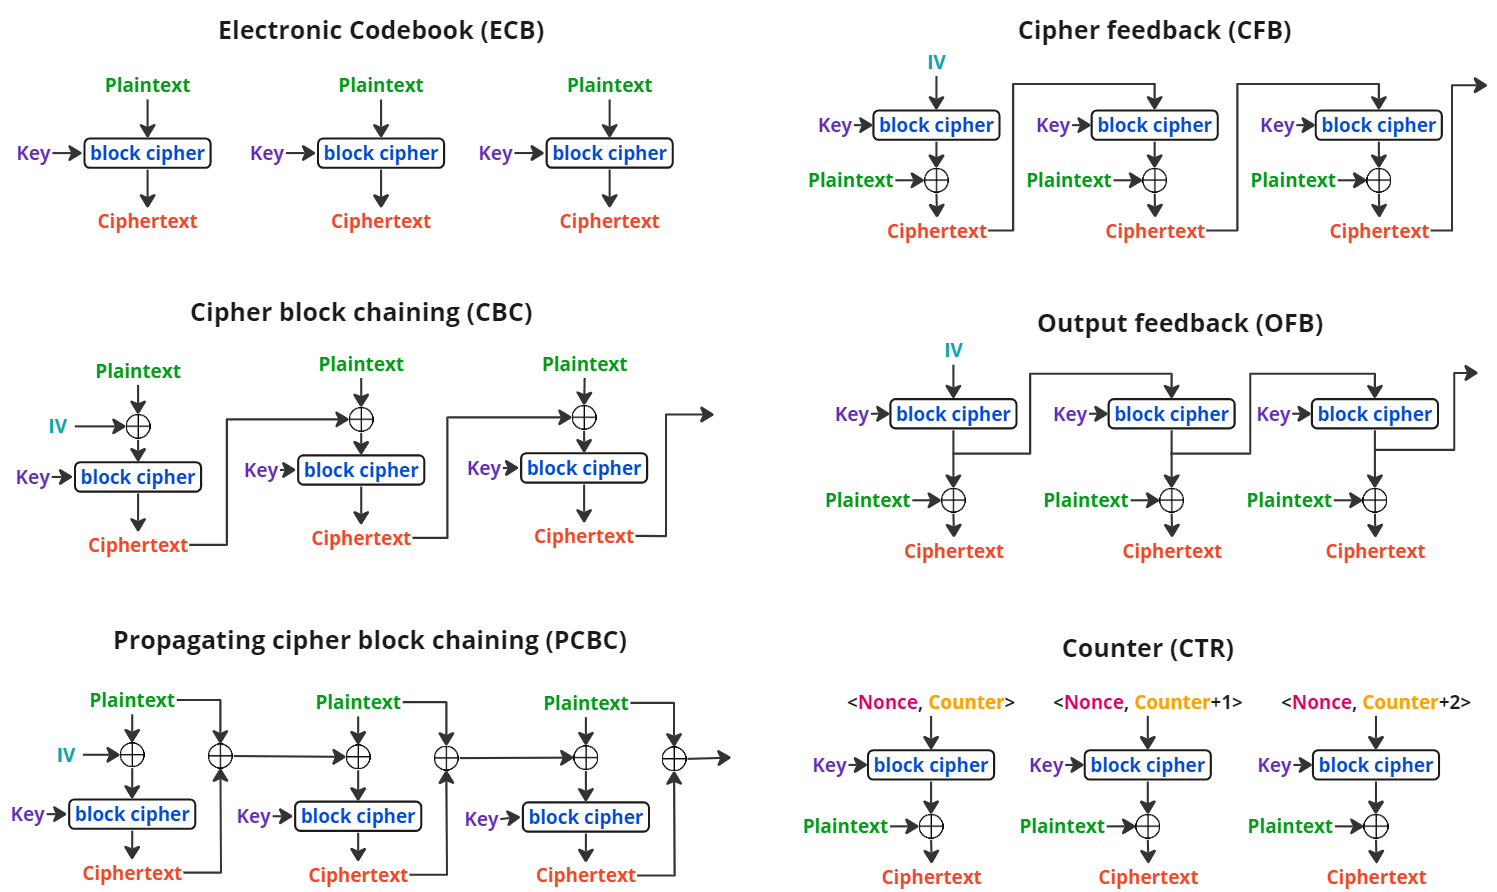
\includegraphics[width=1.1\linewidth]{BlockcipherModesofOperation.png}
    \end{minipage}
    \begin{itemize}
        \item \textit{ECB}: Electronic Code Book, chaque bloc est chiffré séparément
        \item \textit{CBC}: Cipher Block Chaining, chaque bloc est chiffré avec le bloc précédent (vecteur d'initialisation requis)
        \item \textit{GCM}: Galois/Counter Mode, chiffrement par blocs avec authentification
              % TODO: Not exhaustive
    \end{itemize}

    \paragraph{Limitations chiffrement symétrique}
    \begin{itemize}
        \item \textbf{Distribution des clés} Problème de distribution sécurisée des clés.
        \item \textbf{Nombre de clés} Nécessité d'une clé unique pour chaque paire de correspondants.
        \item \textbf{Sécurité des clés} Protection des clés nécessaire contre le vol ou la compromission.
    \end{itemize}

    \paragraph{Diffie-Hellman} Échange de clés sans les échanger (clé publique) $f(x) = g^x \mod p$ avec $g$ et $p$ publics. $x$ et $y$ est choisi aléatoirement par chaque participant.


    \paragraph{Chiffrement Asymétrique} RSA, ECC (Elliptic Curve Cryptography)
    \begin{itemize}
        \item Moins performant que le chiffrement symétrique
        \item Repose sur la difficulté de certains problèmes mathématiques (factorisation pour RSA)
    \end{itemize}
    \subparagraph{RSA} Basé sur la difficulté de factorisation. Connaître une clé ne donne pas d'information sur l'autre clé (clé publique et privée)
    \begin{itemize}
        \item \textbf{Clé Publique} : $(N, e)$
        \item \textbf{Algorithme} :
              \begin{itemize}
                  \item Choisir deux nombres premiers aléatoires $p$ et $q$ de $\frac{l}{2}$ bits avec $l$ la taille du modulus RSA.
                  \item Calculer $N = p \cdot q$ et $\phi(N) = (p-1)(q-1)$.
                  \item Trouver $e$ tel que $1 < e < \phi(N)$ et $e$ premier avec $\phi(N)$.
                  \item Calculer $d$ tel que $d \cdot e \equiv 1 \pmod{\phi(N)}$.
                  \item \textbf{Chiffrement} : $c = m^e \mod N$
                  \item \textbf{Déchiffrement} : $m = c^d \mod N$
              \end{itemize}
              $e$: exposant public, $d$: exposant privé, $N$: modulus, $m$: message, $c$: message chiffré
    \end{itemize}
    \textit{Note:} $e$ ne doit pas avoir de facteur commun avec $\phi(N)$

    \paragraph{Authenticité et Intégrité}
    \subparagraph{MAC} code taille fixe généré par une fonction de hachage (HMAC), permet de prouver origine (authenticité) et vérifier l'intégrité

    \subparagraph{Non-répudiation} Preuve d'origine et de livraison, l'expéditeur ne peut pas nier avoir envoyé le message
    \subparagraph{Signature} Comme MAC avec non-répudiation

    \sep

    \paragraph{Intrusions Logicielles}
    \subparagraph{Memory Overflow} \snum\textcolor{blue!80}{Stack Overflow} écrasement de variables locales, \num\textcolor{blue!80}{Stack Smashing} écrasement avec exécution de code, \num\textcolor{blue!80}{Stack off-by-one} dépassement d'un seul caractère, \num\textcolor{blue!80}{Heap Overflow} écrasement du tas

    \subparagraph{Manipulation d'entiers} \snum\textcolor{blue!80}{Over/Underflow} (Dépassement), \num\textcolor{blue!80}{Signed/Unsigned} (Conversion)
    \subparagraph{Format String} Utilisation de la fonction \texttt{printf} pour lire ou écrire dans la mémoire
    \subparagraph{Contournement des protections mémoire}
    \begin{itemize}
        \item \textbf{Return-to-libc} Exécution de code en appelant des fonctions de la libc
        \item \textbf{Return-oriented programming} Exécution de code en utilisant des fragments de code existants
    \end{itemize}
    \paragraph{Prévention} Stack/heap non-exécutable, randomisation des adressage mémoire (ALSR), libraries sécurisées

    \vspace*{1em}\noindent\begin{minipage}
        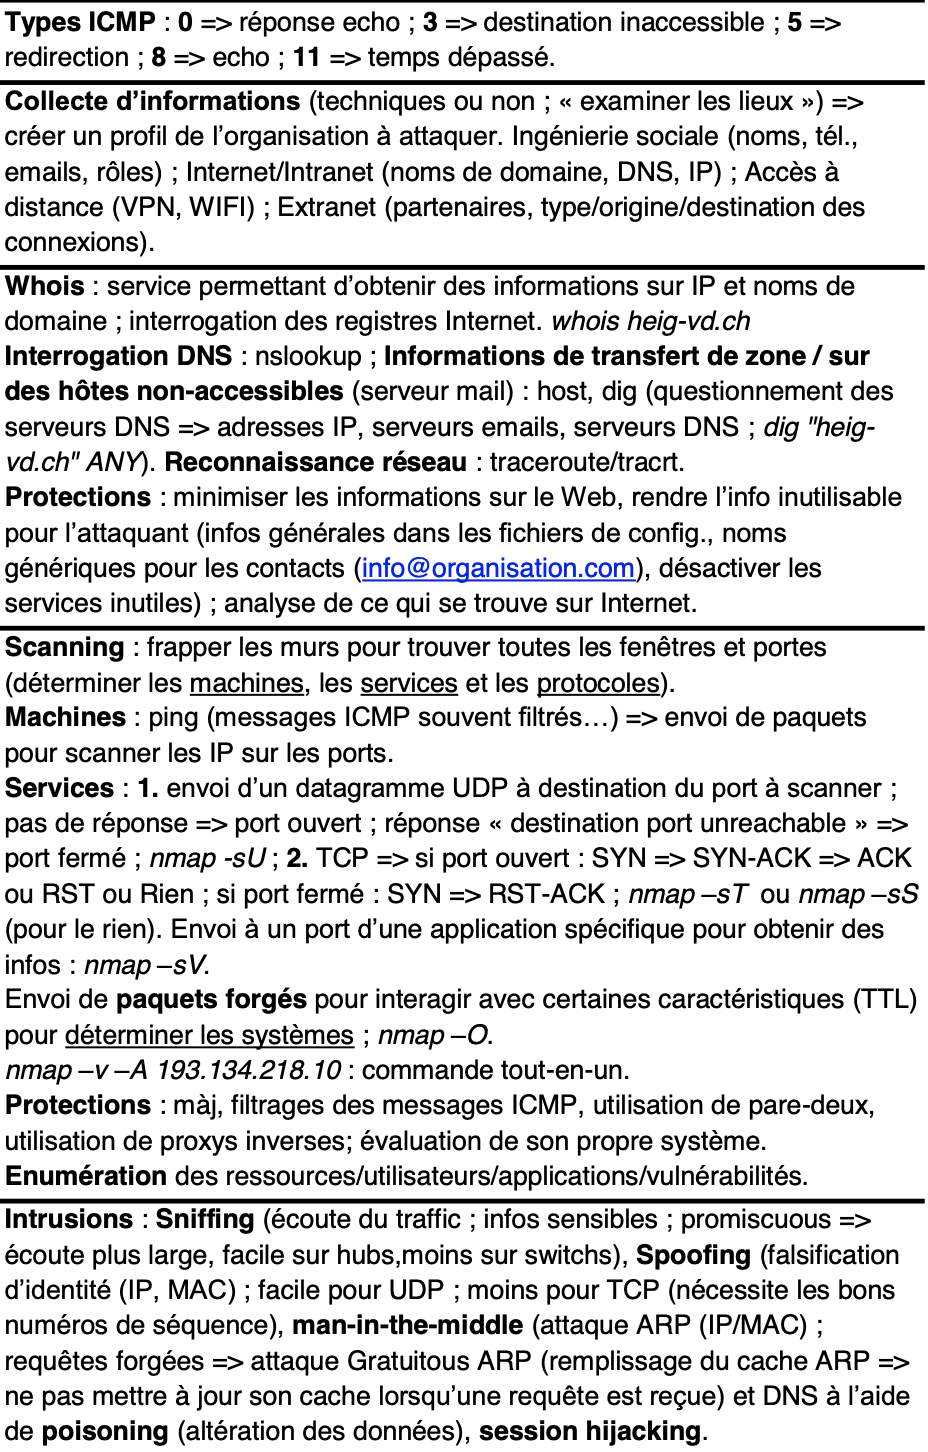
\includegraphics[width=1.1\linewidth]{reseau.png}
    \end{minipage}
\end{multicols*}
\end{document}
